\documentclass[8pt,aspectratio=169]{beamer}
\usetheme{Madrid}
\usepackage{graphicx}
\usepackage{booktabs}
\usepackage{adjustbox}
\usepackage{multicol}
\usepackage{amsmath}
\usepackage{amssymb}
\usepackage{tikz}
\usepackage{hyperref}
\usepackage{algorithm}
\usepackage{algorithmic}
\usepackage{colortbl}
\usepackage{pgfplots}
\pgfplotsset{compat=1.18}

% TikZ libraries for comics, diagrams, stakeholder maps
\usetikzlibrary{arrows.meta,positioning,shapes.callouts,shapes.geometric,decorations.pathreplacing}

% Color definitions
\definecolor{mlblue}{RGB}{0,102,204}
\definecolor{mlpurple}{RGB}{51,51,178}
\definecolor{mllavender}{RGB}{173,173,224}
\definecolor{mllavender2}{RGB}{193,193,232}
\definecolor{mllavender3}{RGB}{204,204,235}
\definecolor{mllavender4}{RGB}{214,214,239}
\definecolor{mlorange}{RGB}{255, 127, 14}
\definecolor{mlgreen}{RGB}{44, 160, 44}
\definecolor{mlred}{RGB}{214, 39, 40}
\definecolor{mlgray}{RGB}{127, 127, 127}
\definecolor{lightgray}{RGB}{240, 240, 240}
\definecolor{midgray}{RGB}{180, 180, 180}

% NEW COLORS for mini-lecture
\definecolor{dfteal}{RGB}{0,128,128}
\definecolor{dfred}{RGB}{180,30,30}

% Backward compatibility
\colorlet{MLPurple}{mlpurple}
\colorlet{MLBlue}{mlblue}
\colorlet{MLOrange}{mlorange}
\colorlet{MLGreen}{mlgreen}
\colorlet{MLRed}{mlred}
\colorlet{MLLavender}{mllavender}
\colorlet{MLGray}{mlgray}

% Theme colors (exact Madrid settings)
\setbeamercolor{palette primary}{bg=mllavender3,fg=mlpurple}
\setbeamercolor{palette secondary}{bg=mllavender2,fg=mlpurple}
\setbeamercolor{palette tertiary}{bg=mllavender,fg=white}
\setbeamercolor{palette quaternary}{bg=mlpurple,fg=white}
\setbeamercolor{structure}{fg=mlpurple}
\setbeamercolor{section in toc}{fg=mlpurple}
\setbeamercolor{subsection in toc}{fg=mlblue}
\setbeamercolor{title}{fg=mlpurple}
\setbeamercolor{frametitle}{fg=mlpurple,bg=mllavender3}
\setbeamercolor{block title}{bg=mllavender2,fg=mlpurple}
\setbeamercolor{block body}{bg=mllavender4,fg=black}
\setbeamertemplate{navigation symbols}{}
\setbeamertemplate{itemize items}[circle]
\setbeamertemplate{enumerate items}[default]
\setbeamersize{text margin left=5mm,text margin right=5mm}

% Footer
\setbeamertemplate{footline}{
  \leavevmode%
  \hbox{%
    \begin{beamercolorbox}[wd=.333333\paperwidth,ht=2.25ex,dp=1ex,center]{author in head/foot}%
      \usebeamerfont{author in head/foot}Methods and Algorithms
    \end{beamercolorbox}%
    \begin{beamercolorbox}[wd=.333333\paperwidth,ht=2.25ex,dp=1ex,center]{title in head/foot}%
      \usebeamerfont{title in head/foot}MSc Data Science
    \end{beamercolorbox}%
    \begin{beamercolorbox}[wd=.333333\paperwidth,ht=2.25ex,dp=1ex,right]{date in head/foot}%
      \usebeamerfont{date in head/foot}\insertframenumber{} / \inserttotalframenumber\hspace*{2ex}
    \end{beamercolorbox}}%
  \vskip0pt%
}

\newcommand{\bottomnote}[1]{%
\vfill
\vspace{-2mm}
\textcolor{mllavender2}{\rule{\textwidth}{0.4pt}}
\vspace{1mm}
\footnotesize
\textbf{#1}
}

\newenvironment{compactlist}{%
  \begin{itemize}%
    \setlength{\itemsep}{2pt}%
    \setlength{\parskip}{0pt}%
    \setlength{\parsep}{0pt}%
}{%
  \end{itemize}%
}

\newcommand{\highlight}[1]{\textcolor{mlorange}{\textbf{#1}}}
\newcommand{\mathbold}[1]{\boldsymbol{#1}}

\title[K-Means Full Lecture]{K-Means Clustering: Theory and Practice}
\subtitle{Full Technical Lecture}
\author{Methods and Algorithms}
\institute{MSc Data Science}
\date{}

\begin{document}

%% ================================================================
%% INTRO ZONE (Slides 1--5, NO formulas)
%% ================================================================

%% SLIDE 1: Title Page
\begin{frame}
\titlepage
\end{frame}

%% SLIDE 2: TikZ Comic Opening
\begin{frame}[t]{A Bank Has 2 Million Customers --- How Do We Group Them?}
\begin{columns}[T]
\column{0.55\textwidth}
\small
\textbf{The Scene}

\footnotesize
A marketing director stares at a customer database with 2 million rows. One-size-fits-all campaigns waste budget.
\begin{compactlist}
\item \footnotesize \textbf{Situation:} 2M customers, diverse behaviors
\item \footnotesize \textbf{Complication:} Generic campaigns get 2\% response rate
\item \footnotesize \textbf{Question:} Can we discover \highlight{natural customer groups}?
\end{compactlist}

\vspace{2mm}
\begin{block}{Core Idea}
\footnotesize What if the data could tell us how many types of customers exist --- and who belongs to each type?
\end{block}

\column{0.42\textwidth}
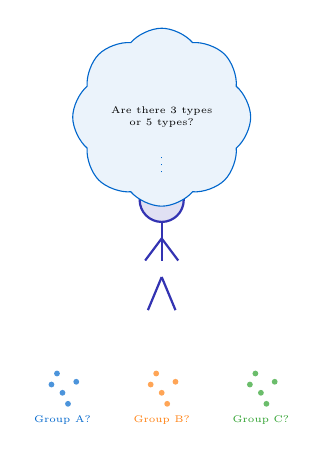
\begin{tikzpicture}[scale=0.7, every node/.style={transform shape}]
% Marketer
\node[circle, draw=mlpurple, fill=mlpurple!15, minimum size=8mm, line width=0.8pt] (head) at (0,4) {};
\node[font=\tiny] at (0,4) {M};
\draw[mlpurple, line width=0.8pt] (head.south) -- ++(0,-0.7);
\draw[mlpurple, line width=0.8pt] (-0.3,2.9) -- (0,3.3) -- (0.3,2.9);
\draw[mlpurple, line width=0.8pt] (0,2.6) -- (-0.25,2.0);
\draw[mlpurple, line width=0.8pt] (0,2.6) -- (0.25,2.0);
% Thought bubble
\node[cloud, draw=mlblue, fill=mlblue!8, cloud puffs=8, cloud puff arc=100,
      minimum width=2.5cm, minimum height=1cm, font=\tiny, align=center] at (0,5.5)
      {Are there 3 types\\or 5 types?};
\draw[mlblue, dotted, line width=0.5pt] (0,4.5) -- (0,4.8);
% Three customer groups
\foreach \x/\c in {-1.8/mlblue, 0/mlorange, 1.8/mlgreen} {
  \foreach \dx/\dy in {0/0, 0.25/0.2, -0.2/0.15, 0.1/-0.2, -0.1/0.35} {
    \fill[\c!70] (\x+\dx, 0.5+\dy) circle (1.5pt);
  }
}
\node[font=\tiny,mlblue] at (-1.8,0) {Group A?};
\node[font=\tiny,mlorange] at (0,0) {Group B?};
\node[font=\tiny,mlgreen] at (1.8,0) {Group C?};
\end{tikzpicture}
\end{columns}
\bottomnote{K-Means discovers structure in unlabeled data --- no predefined groups needed}
\end{frame}

%% SLIDE 3: Learning Objectives
\begin{frame}[t]{What Will You Learn in This Lecture?}
\small
\textbf{Learning Objectives}
\begin{enumerate}
\item \footnotesize \highlight{Derive} the K-Means objective function and analyze its convergence properties
\item \footnotesize \highlight{Evaluate} cluster quality using silhouette scores and the elbow method
\item \footnotesize \highlight{Analyze} how initialization and $K$ selection affect clustering results
\item \footnotesize \highlight{Apply} K-Means to RFM customer segmentation in banking
\end{enumerate}

\vspace{4mm}
\begin{columns}[T]
\column{0.48\textwidth}
\begin{block}{Prerequisites}
\footnotesize Distance metrics, feature scaling (covered in KNN lecture).
\end{block}

\column{0.48\textwidth}
\begin{block}{Why It Matters}
\footnotesize K-Means is the most widely used clustering algorithm in industry --- fast, scalable, and interpretable.
\end{block}
\end{columns}
\bottomnote{Bloom's levels: derive (4), evaluate (5), analyze (4), apply (3)}
\end{frame}

%% SLIDE 4: Plain English Definition
\begin{frame}[t]{What Is K-Means in Plain English?}
\begin{columns}[T]
\column{0.50\textwidth}
\small
\textbf{A simple iterative algorithm}

\footnotesize
Place $K$ centroids. Assign each point to the nearest centroid. Move centroids to the middle of their assigned points. Repeat.
\begin{compactlist}
\item \footnotesize No labels needed --- purely unsupervised
\item \footnotesize Discovers ``natural'' groupings in data
\item \footnotesize Converges in a few iterations typically
\end{compactlist}

\vspace{2mm}
\highlight{Analogy:} ``Placing $K$ magnets on a table of iron filings --- they attract nearby filings and find stable positions.''

\column{0.48\textwidth}
\vspace{2mm}
\footnotesize
\textbf{Key Vocabulary}
\begin{compactlist}
\item \footnotesize \textbf{Centroid:} the center of a cluster ($\boldsymbol{\mu}_k$)
\item \footnotesize \textbf{Cluster:} group of points assigned to one centroid
\item \footnotesize \textbf{Assignment:} mapping each point to nearest centroid
\item \footnotesize \textbf{Iteration:} one assign + update cycle
\item \footnotesize \textbf{Convergence:} centroids stop moving
\end{compactlist}
\end{columns}
\bottomnote{No formulas yet --- K-Means is intuitive: assign, update, repeat}
\end{frame}

%% SLIDE 5: Supervised vs Unsupervised
\begin{frame}[t]{Supervised vs Unsupervised Learning}
\begin{columns}[T]
\column{0.48\textwidth}
\small
\textbf{Supervised Learning}

\footnotesize
\begin{compactlist}
\item \footnotesize \textbf{Input:} features + \highlight{labels}
\item \footnotesize Examples: KNN, logistic regression, decision trees
\item \footnotesize Goal: predict the label of new observations
\item \footnotesize Evaluation: accuracy, precision, recall
\end{compactlist}

\column{0.48\textwidth}
\small
\textbf{Unsupervised Learning}

\footnotesize
\begin{compactlist}
\item \footnotesize \textbf{Input:} features only, \highlight{no labels}
\item \footnotesize Examples: K-Means, PCA, hierarchical clustering
\item \footnotesize Goal: discover structure or groups
\item \footnotesize Evaluation: silhouette, WCSS, domain knowledge
\end{compactlist}
\end{columns}

\vspace{3mm}
\begin{block}{Key Difference}
\footnotesize K-Means doesn't know what the groups \emph{mean} --- it just finds them. \highlight{You} provide the interpretation.
\end{block}
\bottomnote{Unsupervised learning answers: ``What patterns exist?'' not ``What is the label?''}
\end{frame}

%% ================================================================
%% CORE ZONE --- METHOD (Slides 6--14)
%% ================================================================

%% SLIDE 6: K-Means Iteration (Full-size chart)
\begin{frame}[t]{How Does K-Means Iterate?}
\begin{center}

\includegraphics[width=0.65\textwidth]{03_kmeans_iteration/chart}
\end{center}

\vspace{2mm}
\footnotesize
\textcolor{mlblue}{Step 1: Random centroids.}
\quad \textcolor{mlorange}{Step 2: Assign points to nearest centroid.}
\quad \textcolor{mlgreen}{Step 3: Recompute centroids. Repeat.}
\bottomnote{Typically converges in 5--20 iterations for well-separated clusters}
\end{frame}

%% SLIDE 7: Objective Function (Definition block)
\begin{frame}[t]{The K-Means Objective Function}
\begin{block}{Minimize Within-Cluster Sum of Squares (WCSS)}
\[
J = \sum_{k=1}^{K} \sum_{\mathbf{x}_i \in C_k} \|\mathbf{x}_i - \boldsymbol{\mu}_k\|^2
\]
where $\boldsymbol{\mu}_k = \frac{1}{|C_k|}\sum_{\mathbf{x}_i \in C_k} \mathbf{x}_i$ is the centroid of cluster $k$.
\end{block}

\vspace{3mm}
\footnotesize
\highlight{Translation:} Minimize the total squared distance from each point to its cluster center.

\vspace{2mm}
\begin{columns}[T]
\column{0.48\textwidth}
\textbf{Properties:}
\begin{compactlist}
\item \footnotesize $J \geq 0$ always (sum of squares)
\item \footnotesize $J = 0$ only when $K = n$ (each point is its own cluster)
\item \footnotesize Finding global minimum is NP-hard
\end{compactlist}

\column{0.48\textwidth}
\textbf{Lloyd's algorithm finds a local minimum:}
\begin{compactlist}
\item \footnotesize Each step decreases $J$
\item \footnotesize Converges, but not necessarily to global optimum
\item \footnotesize Solution: run multiple times, keep best
\end{compactlist}
\end{columns}
\bottomnote{WCSS is also called ``inertia'' in sklearn}
\end{frame}

%% SLIDE 8: Lloyd's Algorithm (Pseudocode, fragile)
\begin{frame}[fragile,t]{Lloyd's Algorithm Step by Step}
\small
\textbf{The complete K-Means procedure}

\vspace{2mm}
\footnotesize
\begin{semiverbatim}
\textcolor{mlblue}{ALGORITHM:} Lloyd's K-Means

\textcolor{mlblue}{INPUT:}  Data X = \{x_1, ..., x_n\}, number of clusters K
\textcolor{mlblue}{OUTPUT:} Cluster assignments, centroids

1. \textcolor{mlorange}{INITIALIZE} K centroids (randomly or K-Means++)

2. \textcolor{mlorange}{REPEAT:}
   a. \textcolor{mlgreen}{ASSIGN} each point to nearest centroid:
      c_i = argmin_k ||x_i - mu_k||^2

   b. \textcolor{mlgreen}{UPDATE} centroids to cluster means:
      mu_k = (1/|C_k|) * sum(x_i for x_i in C_k)

3. \textcolor{mlorange}{UNTIL} centroids don't change (or max iterations)
\end{semiverbatim}

\vspace{2mm}
\begin{block}{Convergence Guarantee}
\footnotesize Each step decreases $J$ $\to$ algorithm \highlight{must} converge (monotone + bounded below).
\end{block}
\bottomnote{Lloyd (1982) --- one of the most-cited algorithms in computer science}
\end{frame}

%% SLIDE 9: Worked Numerical Example (Chart + table)
\begin{frame}[t]{Worked Example: Clustering 6 Customers}
\begin{columns}[T]
\column{0.50\textwidth}
\begin{center}

\includegraphics[width=\textwidth]{12_kmeans_worked_example/chart}
\end{center}

\column{0.48\textwidth}
\footnotesize
\textbf{6 customers:} Age, Income (k\euro{})

\vspace{1mm}
\begin{tabular}{ccc}
\toprule
\textbf{ID} & \textbf{Age} & \textbf{Income} \\
\midrule
A & 25 & 30 \\
B & 28 & 35 \\
C & 30 & 32 \\
D & 45 & 70 \\
E & 50 & 65 \\
F & 48 & 75 \\
\bottomrule
\end{tabular}

\vspace{2mm}
\textbf{Init} ($K{=}2$): $\mu_1{=}(25,30)$, $\mu_2{=}(45,70)$

\vspace{1mm}
\textbf{Iter 1:} $C_1{=}\{A,B,C\}$, $C_2{=}\{D,E,F\}$

$\mu_1{=}(27.7, 32.3)$, $\mu_2{=}(47.7, 70.0)$

\vspace{1mm}
\textbf{Iter 2:} Same assignments $\to$ \highlight{converged!}

WCSS: $37.3 + 52.7 = 90.0$
\end{columns}
\bottomnote{In practice, K-Means often converges in fewer than 10 iterations}
\end{frame}

%% SLIDE 10: Initialization (Two-column)
\begin{frame}[t]{Why Does Initialization Matter?}
\begin{columns}[T]
\column{0.48\textwidth}
\small
\textcolor{mlred}{\textbf{Bad Initialization}}

\footnotesize
\begin{compactlist}
\item \footnotesize Centroids start close together
\item \footnotesize Algorithm gets stuck in local minimum
\item \footnotesize WCSS much higher than optimal
\item \footnotesize Different runs give different results
\end{compactlist}

\vspace{2mm}
\textbf{Naive approach:} pick $K$ random data points.

Problem: may pick $K$ points from the same cluster.

\column{0.48\textwidth}
\small
\textcolor{mlgreen}{\textbf{K-Means++ Initialization}}

\footnotesize
\begin{enumerate}
\item \footnotesize Pick first centroid randomly
\item \footnotesize Next centroid: probability $\propto d(\mathbf{x}, \text{nearest centroid})^2$
\item \footnotesize Repeat until $K$ centroids chosen
\end{enumerate}

\vspace{2mm}
\textbf{Effect:} Spreads centroids far apart $\to$ better convergence, lower WCSS.

\vspace{2mm}
\begin{block}{sklearn Default}
\footnotesize \texttt{init='k-means++'} + \texttt{n\_init=10} (runs 10 times, keeps best).
\end{block}
\end{columns}
\bottomnote{Arthur \& Vassilvitskii (2007) --- K-Means++ guarantees $O(\log K)$-competitive WCSS}
\end{frame}

%% SLIDE 11: Voronoi Diagrams (Chart + text)
\begin{frame}[t]{What Shape Are K-Means Clusters?}
\begin{columns}[T]
\column{0.55\textwidth}
\begin{center}

\includegraphics[width=\textwidth]{06_voronoi/chart}
\end{center}

\column{0.43\textwidth}
\small
\textbf{Voronoi Cells}

\footnotesize
Each point belongs to the region of the nearest centroid. These regions form \highlight{Voronoi cells}.
\begin{compactlist}
\item \footnotesize Cells are always \textbf{convex polygons}
\item \footnotesize Boundaries are perpendicular bisectors
\item \footnotesize Clusters are roughly spherical
\end{compactlist}

\vspace{2mm}
\textcolor{mlred}{\textbf{Limitation:}}
\begin{compactlist}
\item \footnotesize Cannot capture elongated shapes
\item \footnotesize Cannot capture ring/crescent clusters
\item \footnotesize Cannot handle very different cluster sizes
\end{compactlist}
\end{columns}
\bottomnote{Voronoi diagrams appear throughout computational geometry and spatial analysis}
\end{frame}

%% SLIDE 12: Convergence Proof Sketch
\begin{frame}[t]{Why Must K-Means Converge?}
\begin{columns}[T]
\column{0.48\textwidth}
\small
\textbf{Step 1: Assignment decreases $J$}

\footnotesize
For fixed centroids $\boldsymbol{\mu}_k$, assigning each point to its \highlight{nearest} centroid minimizes:
\[
J_{\text{assign}} = \sum_{i=1}^{n} \|\mathbf{x}_i - \boldsymbol{\mu}_{c_i}\|^2
\]
Any other assignment would increase $J$.

\column{0.48\textwidth}
\small
\textbf{Step 2: Update decreases $J$}

\footnotesize
For fixed assignments, the \highlight{mean} minimizes sum of squared distances:
\[
\boldsymbol{\mu}_k^* = \arg\min_{\boldsymbol{\mu}} \sum_{\mathbf{x}_i \in C_k} \|\mathbf{x}_i - \boldsymbol{\mu}\|^2
\]
The mean is the unique minimizer (convex optimization).
\end{columns}

\vspace{3mm}
\begin{block}{Convergence Argument}
\footnotesize
Both steps \highlight{decrease} (or maintain) $J$. Since $J \geq 0$, the sequence $J^{(1)}, J^{(2)}, \ldots$ is monotone decreasing and bounded below $\to$ must converge. \textcolor{mlred}{But:} convergence to \emph{global} optimum is NOT guaranteed.
\end{block}
\bottomnote{Practical fix: run K-Means multiple times with different initializations (\texttt{n\_init=10})}
\end{frame}

%% SLIDE 13: Choosing K --- Elbow Method (Chart + methods)
\begin{frame}[t]{How Do We Choose $K$?}
\begin{columns}[T]
\column{0.55\textwidth}
\begin{center}

\includegraphics[width=\textwidth]{04_elbow_method/chart}
\end{center}

\column{0.43\textwidth}
\small
\textbf{Three Methods}

\footnotesize
\textcolor{mlblue}{\textbf{1. Elbow method:}}
\begin{compactlist}
\item \footnotesize Plot WCSS vs $K$
\item \footnotesize Find the ``elbow'' where improvement slows
\end{compactlist}

\vspace{2mm}
\textcolor{mlorange}{\textbf{2. Silhouette score:}}
\begin{compactlist}
\item \footnotesize Measures how well-separated clusters are
\item \footnotesize Pick $K$ that maximizes mean silhouette
\end{compactlist}

\vspace{2mm}
\textcolor{mlgreen}{\textbf{3. Domain knowledge:}}
\begin{compactlist}
\item \footnotesize ``Our bank wants 4 product tiers'' $\to$ $K{=}4$
\item \footnotesize Business constraints often dictate $K$
\end{compactlist}
\end{columns}
\bottomnote{No single method is perfect --- combine quantitative metrics with business judgment}
\end{frame}

%% SLIDE 14: Silhouette Score (Chart + formula)
\begin{frame}[t]{What Does the Silhouette Score Tell Us?}
\begin{columns}[T]
\column{0.55\textwidth}
\begin{center}

\includegraphics[width=\textwidth]{05_silhouette/chart}
\end{center}

\column{0.43\textwidth}
\small
\textbf{Silhouette Score}

\footnotesize
For each point $i$:
\begin{compactlist}
\item \footnotesize $a(i)$ = mean distance to own cluster
\item \footnotesize $b(i)$ = mean distance to nearest other cluster
\end{compactlist}

\[
s(i) = \frac{b(i) - a(i)}{\max(a(i),\; b(i))} \in [-1, 1]
\]

\vspace{2mm}
\textbf{Interpretation:}
\begin{compactlist}
\item \footnotesize $s \approx 1$: well-clustered
\item \footnotesize $s \approx 0$: on cluster boundary
\item \footnotesize $s < 0$: likely in wrong cluster
\end{compactlist}
\end{columns}
\bottomnote{Average silhouette $> 0.5$ is generally considered good clustering}
\end{frame}

%% ================================================================
%% CORE ZONE --- SOLUTION (Slides 15--19)
%% ================================================================

%% SLIDE 15: RFM Segmentation (Chart + text)
\begin{frame}[t]{RFM Segmentation: A Real Banking Application}
\begin{columns}[T]
\column{0.55\textwidth}
\begin{center}

\includegraphics[width=\textwidth]{11_rfm_scatter/chart}
\end{center}

\column{0.43\textwidth}
\small
\textbf{RFM Features}

\footnotesize
\begin{compactlist}
\item \footnotesize \textbf{R}ecency: days since last transaction
\item \footnotesize \textbf{F}requency: transactions per month
\item \footnotesize \textbf{M}onetary: average transaction amount
\end{compactlist}

\vspace{2mm}
\textbf{Discovered Segments:}
\begin{compactlist}
\item \footnotesize \textcolor{mlblue}{\textbf{High-value loyal:}} low R, high F, high M
\item \footnotesize \textcolor{mlred}{\textbf{Dormant:}} high R, low F, low M
\item \footnotesize \textcolor{mlgreen}{\textbf{Active small:}} low R, high F, low M
\end{compactlist}

\vspace{2mm}
\highlight{Each segment gets a tailored marketing strategy.}
\end{columns}
\bottomnote{RFM segmentation is standard practice in retail banking and e-commerce}
\end{frame}

%% SLIDE 16: Interpreting Cluster Centers (Table)
\begin{frame}[t]{Interpreting Cluster Centers}
\small
\textbf{The centroid IS the cluster prototype}

\vspace{3mm}
\footnotesize
\begin{tabular}{clccc}
\toprule
\textbf{Cluster} & \textbf{Segment Name} & \textbf{Recency (days)} & \textbf{Frequency (/month)} & \textbf{Monetary (\euro{})} \\
\midrule
1 & High-value loyal & 5 & 28 & 2,400 \\
2 & Dormant & 120 & 2 & 150 \\
3 & Active small spenders & 8 & 22 & 180 \\
\bottomrule
\end{tabular}

\vspace{4mm}
\textbf{Marketing actions:}
\begin{compactlist}
\item \footnotesize \textcolor{mlblue}{\textbf{Cluster 1:}} Premium rewards, exclusive offers, retention priority
\item \footnotesize \textcolor{mlred}{\textbf{Cluster 2:}} Win-back campaign, special reactivation discount
\item \footnotesize \textcolor{mlgreen}{\textbf{Cluster 3:}} Upsell opportunities, loyalty program enrollment
\end{compactlist}

\vspace{3mm}
\begin{block}{New Customer Assignment}
\footnotesize Compare a new customer's RFM values to each centroid $\to$ assign to nearest $\to$ apply that segment's strategy.
\end{block}
\bottomnote{Centroids provide interpretable cluster summaries --- show them to business stakeholders}
\end{frame}

%% SLIDE 17: When K-Means Fails (Two-column with TikZ)
\begin{frame}[t]{When Does K-Means Fail?}
\begin{columns}[T]
\column{0.48\textwidth}
\small
\textcolor{mlred}{\textbf{K-Means Fails When Clusters Are:}}

\footnotesize
\begin{compactlist}
\item \footnotesize \textbf{Non-spherical:} elongated, ring-shaped, crescent
\item \footnotesize \textbf{Very different sizes:} large cluster absorbs small ones
\item \footnotesize \textbf{Different densities:} sparse cluster merged with dense
\end{compactlist}

\vspace{2mm}
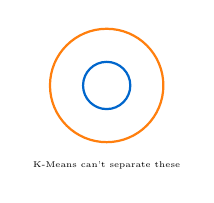
\begin{tikzpicture}[scale=0.6, every node/.style={transform shape}]
% Two concentric circles
\draw[mlblue, thick] (0,0) circle (0.5);
\draw[mlorange, thick] (0,0) circle (1.2);
\node[font=\tiny, below] at (0,-1.5) {K-Means can't separate these};
\end{tikzpicture}

\column{0.48\textwidth}
\small
\textcolor{mlgreen}{\textbf{Alternatives}}

\footnotesize
\begin{compactlist}
\item \footnotesize \textbf{DBSCAN:} density-based, no $K$ needed, arbitrary shapes
\item \footnotesize \textbf{Gaussian Mixtures:} soft assignment, elliptical clusters
\item \footnotesize \textbf{Hierarchical:} dendrogram reveals cluster hierarchy
\item \footnotesize \textbf{Spectral clustering:} graph-based, handles non-convex
\end{compactlist}

\vspace{2mm}
\begin{block}{Rule of Thumb}
\footnotesize If clusters look roughly spherical and equally sized $\to$ K-Means. Otherwise $\to$ consider alternatives.
\end{block}
\end{columns}
\bottomnote{No single clustering algorithm works for all data shapes --- know the assumptions}
\end{frame}

%% SLIDE 18: K-Means vs GMM (Comparison)
\begin{frame}[t]{K-Means and Gaussian Mixture Models}
\begin{columns}[T]
\column{0.48\textwidth}
\small
\textbf{K-Means = Hard Assignment}

\footnotesize
\begin{compactlist}
\item \footnotesize Each point belongs to \highlight{exactly one} cluster
\item \footnotesize Cluster shapes: spherical only
\item \footnotesize Objective: minimize WCSS
\item \footnotesize Fast, simple, deterministic (given init)
\end{compactlist}

\column{0.48\textwidth}
\small
\textbf{GMM = Soft Assignment}

\footnotesize
\begin{compactlist}
\item \footnotesize Each point has a \highlight{probability} per cluster
\item \footnotesize Cluster shapes: elliptical (full covariance)
\item \footnotesize Objective: maximize likelihood via EM
\item \footnotesize More flexible, slower
\end{compactlist}
\end{columns}

\vspace{3mm}
\begin{block}{Connection}
\footnotesize K-Means is a special case of EM for Gaussian mixtures with \highlight{equal, spherical covariances}. Understanding K-Means builds intuition for GMMs.
\end{block}

\vspace{2mm}
\footnotesize
\textbf{Preview:} Soft assignments connect to embeddings (L06) and probabilistic models in later courses.
\bottomnote{GMM: \texttt{sklearn.mixture.GaussianMixture(n\_components=K)}}
\end{frame}

%% SLIDE 19: Computational Complexity (Two-column)
\begin{frame}[t]{Computational Complexity}
\begin{columns}[T]
\column{0.48\textwidth}
\small
\textbf{K-Means Complexity}

\footnotesize
$O(n \times K \times p \times I)$ per run
\begin{compactlist}
\item \footnotesize $n$ = number of points
\item \footnotesize $K$ = number of clusters
\item \footnotesize $p$ = number of features
\item \footnotesize $I$ = number of iterations (typically 5--20)
\end{compactlist}

\vspace{2mm}
\highlight{Very fast} --- handles millions of points on a laptop.

\column{0.48\textwidth}
\small
\textbf{Comparison}

\footnotesize
\begin{tabular}{ll}
\toprule
\textbf{Algorithm} & \textbf{Complexity} \\
\midrule
K-Means & $O(nKpI)$ \\
DBSCAN & $O(n \log n)$ \\
Hierarchical & $O(n^2 \log n)$ \\
GMM (EM) & $O(nKp^2 I)$ \\
\bottomrule
\end{tabular}

\vspace{2mm}
K-Means scales \textbf{linearly} with $n$. Hierarchical clustering is $O(n^2)$ --- doesn't scale.
\end{columns}

\vspace{3mm}
\begin{block}{Mini-Batch K-Means}
\footnotesize For very large datasets: use random subsamples per iteration. \texttt{MiniBatchKMeans} in sklearn.
\end{block}
\bottomnote{K-Means is the fastest clustering algorithm for large-scale applications}
\end{frame}

%% ================================================================
%% CLOSING ZONE (Slides 20--25)
%% ================================================================

%% SLIDE 20: Pros and Cons
\begin{frame}[t]{When to Use K-Means --- and When Not To}
\begin{columns}[T]
\column{0.48\textwidth}
\small
\textcolor{mlgreen}{\textbf{Strengths}}

\footnotesize
\begin{compactlist}
\item \footnotesize \textcolor{mlgreen}{\checkmark} Fast and scalable (linear in $n$)
\item \footnotesize \textcolor{mlgreen}{\checkmark} Easy to interpret (centroids = prototypes)
\item \footnotesize \textcolor{mlgreen}{\checkmark} Works well on spherical clusters
\item \footnotesize \textcolor{mlgreen}{\checkmark} Simple to implement and parallelize
\item \footnotesize \textcolor{mlgreen}{\checkmark} Guaranteed convergence
\end{compactlist}

\column{0.48\textwidth}
\small
\textcolor{mlred}{\textbf{Limitations}}

\footnotesize
\begin{compactlist}
\item \footnotesize \textcolor{mlred}{$\times$} Must specify $K$ in advance
\item \footnotesize \textcolor{mlred}{$\times$} Sensitive to initialization
\item \footnotesize \textcolor{mlred}{$\times$} Assumes spherical, equal-size clusters
\item \footnotesize \textcolor{mlred}{$\times$} Sensitive to outliers (they pull centroids)
\item \footnotesize \textcolor{mlred}{$\times$} Only finds local optimum
\end{compactlist}
\end{columns}

\vspace{3mm}
\begin{block}{Rule of Thumb}
\footnotesize Use K-Means when: spherical clusters expected, need fast results, have domain knowledge for $K$. Avoid when: unknown cluster shapes, many outliers, need probabilistic assignments.
\end{block}
\bottomnote{K-Means is an excellent starting point --- always try it first before complex methods}
\end{frame}

%% SLIDE 21: K-Means vs DBSCAN vs Hierarchical (Comparison table)
\begin{frame}[t]{K-Means vs DBSCAN vs Hierarchical Clustering}
\small
\vspace{1mm}
\footnotesize
\begin{tabular}{llll}
\toprule
\textbf{Criterion} & \textbf{K-Means} & \textbf{DBSCAN} & \textbf{Hierarchical} \\
\midrule
$K$ required? & \textcolor{mlred}{Yes} & \textcolor{mlgreen}{No} & Cut dendrogram \\
Cluster shapes & Spherical only & \textcolor{mlgreen}{Arbitrary} & Arbitrary \\
Scalability & \textcolor{mlgreen}{$O(nKpI)$} & $O(n \log n)$ & \textcolor{mlred}{$O(n^2)$} \\
Outlier handling & \textcolor{mlred}{Poor} & \textcolor{mlgreen}{Built-in} & Moderate \\
Interpretability & Centroids & Core/border pts & Dendrogram \\
Deterministic? & No (init) & \textcolor{mlgreen}{Yes} & \textcolor{mlgreen}{Yes} \\
\bottomrule
\end{tabular}

\vspace{3mm}
\begin{block}{When to Choose Which?}
\footnotesize
\textbf{K-Means:} Large data, spherical clusters, known $K$. \quad
\textbf{DBSCAN:} Unknown $K$, arbitrary shapes, outliers. \quad
\textbf{Hierarchical:} Small data, want to explore cluster hierarchy.
\end{block}
\bottomnote{In practice, try K-Means first for speed, then DBSCAN if K-Means clusters look wrong}
\end{frame}

%% SLIDE 22: Code Example (fragile frame)
\begin{frame}[fragile,t]{Hands-On: Segment Bank Customers}
\small
\textbf{Complete sklearn workflow}

\vspace{2mm}
\footnotesize
\begin{semiverbatim}
\textcolor{mlblue}{import} numpy \textcolor{mlblue}{as} np
\textcolor{mlblue}{from} sklearn.cluster \textcolor{mlblue}{import} KMeans
\textcolor{mlblue}{from} sklearn.preprocessing \textcolor{mlblue}{import} StandardScaler
\textcolor{mlblue}{from} sklearn.metrics \textcolor{mlblue}{import} silhouette_score

\textcolor{mlgray}{# Step 1: Scale RFM features}
scaler = StandardScaler()
X_scaled = scaler.fit_transform(X_rfm)

\textcolor{mlgray}{# Step 2: Fit K-Means}
kmeans = KMeans(n_clusters=4, n_init=10, random_state=42)
labels = kmeans.fit_predict(X_scaled)

\textcolor{mlgray}{# Step 3: Evaluate}
print(f\textcolor{mlorange}{"Cluster sizes: \{np.bincount(labels)\}"})
print(f\textcolor{mlorange}{"Silhouette:    \{silhouette_score(X_scaled, labels):.3f\}"})
print(f\textcolor{mlorange}{"WCSS:          \{kmeans.inertia_:.1f\}"})
\end{semiverbatim}

\vspace{2mm}
\footnotesize
Full notebook: \texttt{L03\_kmeans.ipynb} on Colab
\bottomnote{Always scale features before K-Means --- distance-based methods require comparable scales}
\end{frame}

%% SLIDE 23: Key Takeaways (Two-column summary)
\begin{frame}[t]{Key Takeaways}
\begin{columns}[T]
\column{0.48\textwidth}
\small
\textcolor{mlpurple}{\textbf{Concepts}}

\footnotesize
\begin{compactlist}
\item \footnotesize WCSS objective function
\item \footnotesize Lloyd's algorithm (assign + update)
\item \footnotesize Convergence guarantee (monotone + bounded)
\item \footnotesize K-Means++ initialization
\item \footnotesize Silhouette score and elbow method
\item \footnotesize Voronoi cells and spherical assumption
\end{compactlist}

\column{0.48\textwidth}
\small
\textcolor{mlpurple}{\textbf{Practice}}

\footnotesize
\begin{compactlist}
\item \footnotesize \highlight{Always} scale features before clustering
\item \footnotesize Use K-Means++ init (\texttt{init='k-means++'})
\item \footnotesize Try multiple $K$ values (elbow + silhouette)
\item \footnotesize Run multiple times (\texttt{n\_init=10})
\item \footnotesize Combine metrics with domain knowledge
\item \footnotesize Inspect centroids for business interpretation
\end{compactlist}
\end{columns}

\vspace{3mm}
\begin{block}{One Sentence Summary}
\footnotesize K-Means partitions data into $K$ groups by iteratively minimizing within-cluster distances --- fast, interpretable, and the go-to algorithm for large-scale clustering.
\end{block}
\bottomnote{K-Means is the starting point for all clustering tasks in industry}
\end{frame}

%% SLIDE 24: Bridge to Next Lecture
\begin{frame}[t]{What's Next: Decision Trees and Random Forests}
\small
\textbf{From distance-based to rule-based learning}

\vspace{3mm}
\footnotesize
\begin{columns}[T]
\column{0.48\textwidth}
\textbf{What we covered (L03):}
\begin{compactlist}
\item \footnotesize \textbf{KNN:} distance + labels $\to$ classify
\item \footnotesize \textbf{K-Means:} distance + no labels $\to$ cluster
\item \footnotesize Both rely on ``closeness'' in feature space
\end{compactlist}

\column{0.48\textwidth}
\textbf{What's coming (L04):}
\begin{compactlist}
\item \footnotesize \textbf{Decision Trees:} learn \highlight{rules}, not distances
\item \footnotesize Questions like ``Is income $> 50$k?''
\item \footnotesize Foundation for Random Forests and XGBoost
\end{compactlist}
\end{columns}

\vspace{4mm}
\begin{block}{Preview}
\footnotesize Decision trees discover the best sequence of yes/no questions to split data --- replacing distance with information gain.
\end{block}
\bottomnote{Next lecture: from ``who is closest?'' to ``what is the best question to ask?''}
\end{frame}

%% SLIDE 25: XKCD Closing
\begin{frame}[t]{Closing Thought}
\begin{center}
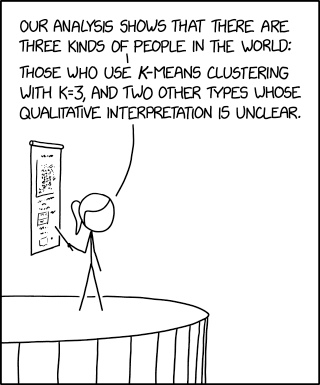
\includegraphics[height=0.55\textheight]{images/2731_kmeans_clustering.png}
\end{center}
\vspace{-1mm}
\footnotesize
\begin{center}
\emph{``Unsupervised learning finds what you didn't know to look for.''}
\end{center}
\bottomnote{XKCD \#2731 by Randall Munroe (CC BY-NC 2.5)}
\end{frame}

\end{document}
